\documentclass[a4paper,11pt]{article}
\usepackage[ngerman]{babel}
\usepackage[ansinew]{inputenc}
\usepackage{geometry}
\usepackage{graphicx}
\usepackage{ulem}
\usepackage{listings}

\geometry{top=20mm, left=30mm, right=30mm, bottom=20mm}
\parindent 0pt
\lstset{language=SQL} 


\title{Dokumentation zum Datenbankprojekt}
\author{Katharina Chowanski / Marvin Kleinert / Marius Schidlack}  
\date{\today}

\begin{document}
\maketitle 

\section*{Iteration 1: Modellierung}
\begin{enumerate}
\item Entity-Relationship-Modell
\begin{figure}[htbp]
	\centering
		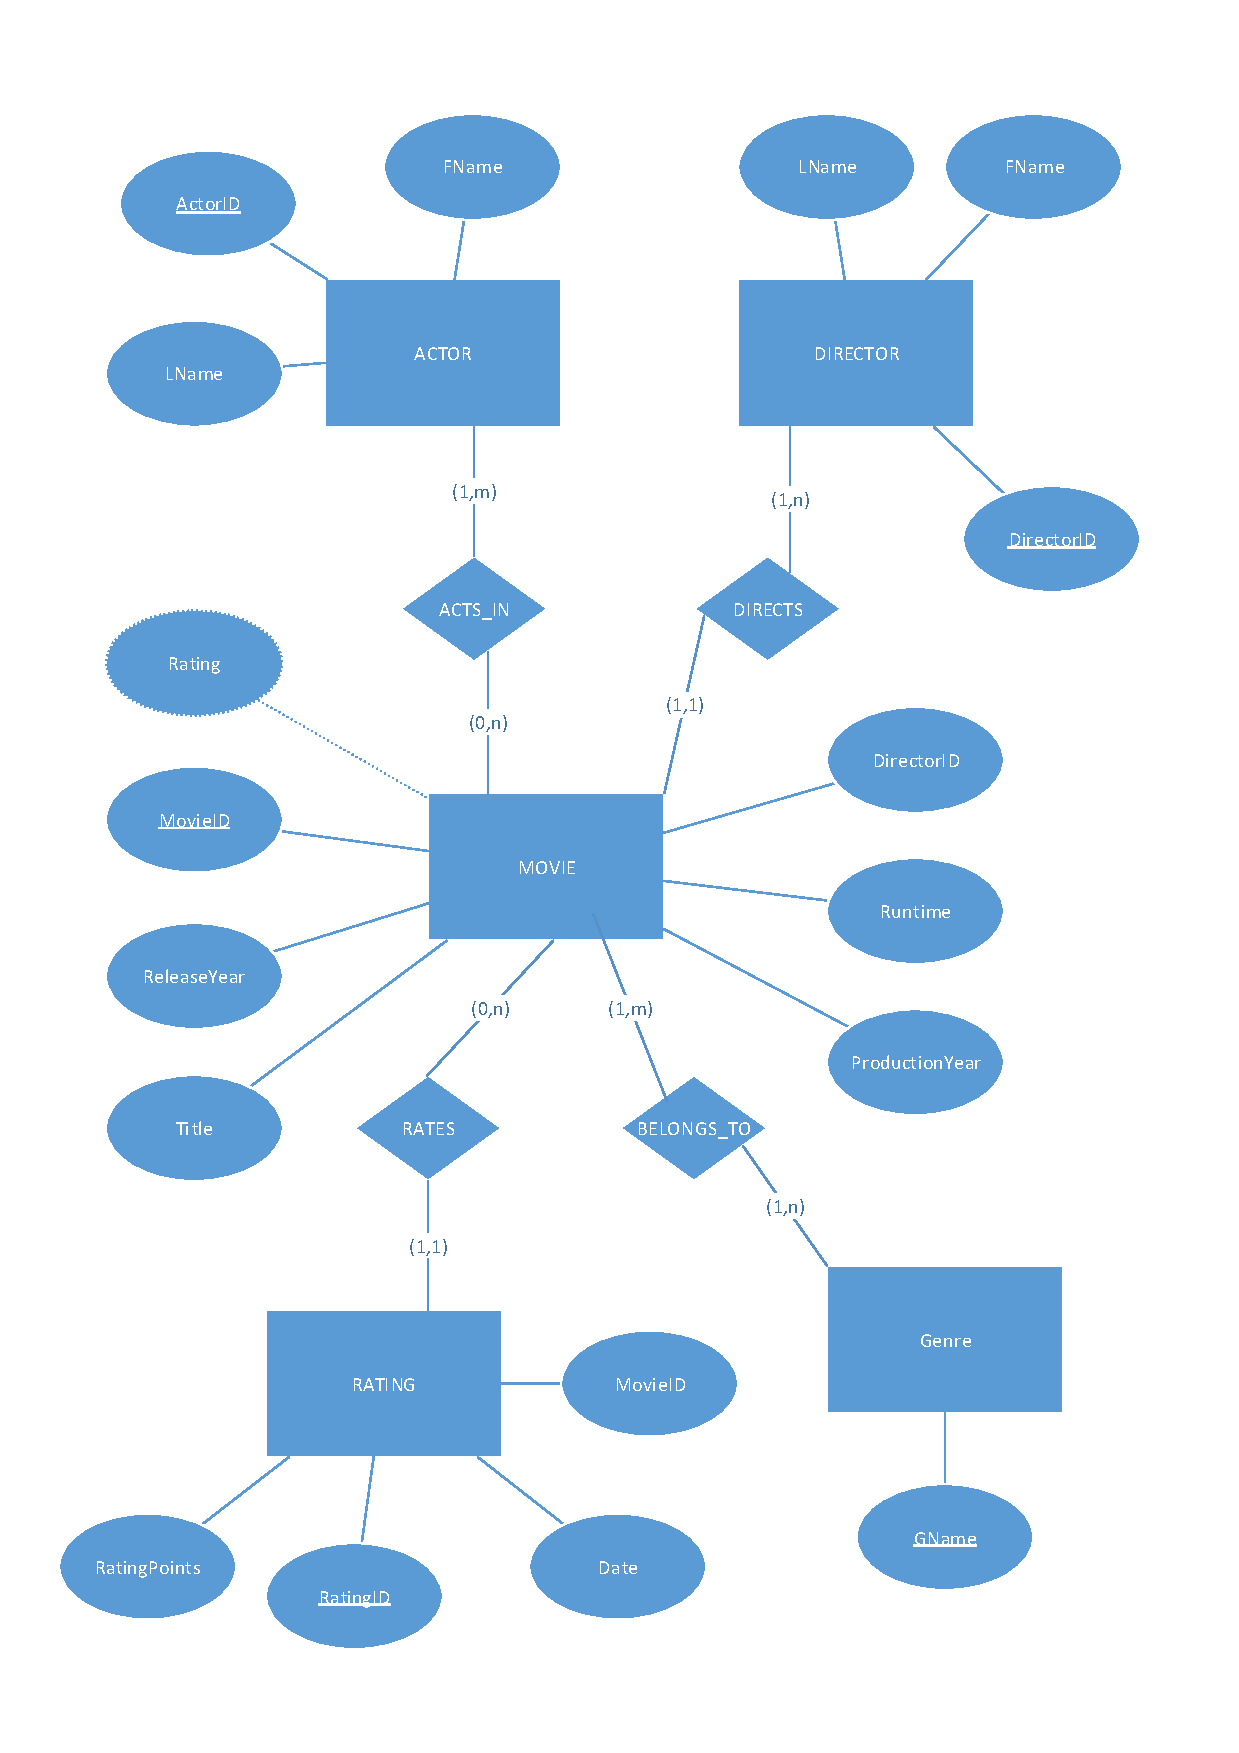
\includegraphics[width=0.85\textwidth]{MoviesER_Portrait.pdf}
	\label{fig:MoviesER}
\end{figure}

\item Relationales Modell \\[0.5cm]
MOVIE (Title: string; \uline{MovieID}: int; ReleaseYear: int; ProductionYear: int; Runtime: int; DirectorID: int; Rating: float)\\[0.5cm]
ACTOR (\uline{ActorID}: int; FName: string; Lname: string)\\[0.5cm]
DIRECTOR (\uline{DirectorID}: int; FName: string; LName: string)\\[0.5cm]
RATING (\uline{RatingID}: int; Date: date; RatingPoints: int; MovieID: int)\\[0.5cm]
GENRE (\uline{GName}: string)\\[0.5cm]
ACTS\_IN (\underline{\dashuline{MovieID}}: int; \underline{\dashuline{ActorID}}: int)\\[0.5cm]
BELONGS\_TO (\underline{\dashuline{GName}}: string; \underline{\dashuline{MovieID}}: int)\\[0.5cm]

\item CREATE-Statements
\begin{lstlisting}
CREATE TABLE MOVIE 
(Title				varchar(255) NOT NULL,
MovieID				int8 NOT NULL,
ReleaseYear			interval YEAR,
ProductionYear			interval YEAR,
Runtime				int4,
DirectorID			int8 NOT NULL,
Rating				float4,
PRIMARY KEY (MovieID),
FOREIGN KEY (DirectorID) REFERENCES DIRECTOR (DirectorID)
);

CREATE TABLE ACTOR
(ActorID			int8 NOT NULL,
FName				varchar(255),
LName				varchar(255),
PRIMARY KEY (ActorID)
);

CREATE TABLE DIRECTOR
(DirectorID			int8 NOT NULL,
FName				varchar(255),
LName 				varchar(255),
PRIMARY KEY (DirectorID)
);

CREATE TABLE RATING
(RatingID			int8 NOT NULL,
Date				date,
RatingPoints			int4,
MovieID				int8 NOT NULL,
PRIMARY KEY (RatingID),
FOREIGN KEY (MovieID) REFERENCES MOVIE (MovieID)
);

CREATE TABLE GENRE
(GName				varchar(255) NOT NULL,
PRIMARY KEY (GName)
);

CREATE TABLE ACTS_IN
(MovieID			int8 NOT NULL,
ActorID				int8 NOT NULL,
PRIMARY KEY (MovieID, ActorID),
FOREIGN KEY (MovieID) REFERENCES MOVIE(MovieID),
FOREIGN KEY (ActorID) REFERENCES ACTOR (ActorID)
);

CREATE TABLE BELONGS_TO
(GName				varchar(255) NOT NULL,
MovieID				int8 NOT NULL,
PRIMARY KEY (GName, MovieID),
FOREIGN KEY (GName) REFERENCES GENRE (GName),
FOREIGN KEY (MovieID) REFERENCES MOVIE (MovieID)
);


\end{lstlisting}
\end{enumerate}

\end{document}